\begin{frame}{Evaluation}
    \begin{itemize}
      \item Rust wird mit C und X10 verglichen
      \item Wiederholte Laufzeitmessungen
      \item Betrachtung von Programmen mit und ohne Compiler-Optimierungen
    \end{itemize}
\end{frame}

\begin{frame}{Kompilierungsdauer}
  \begin{center}
    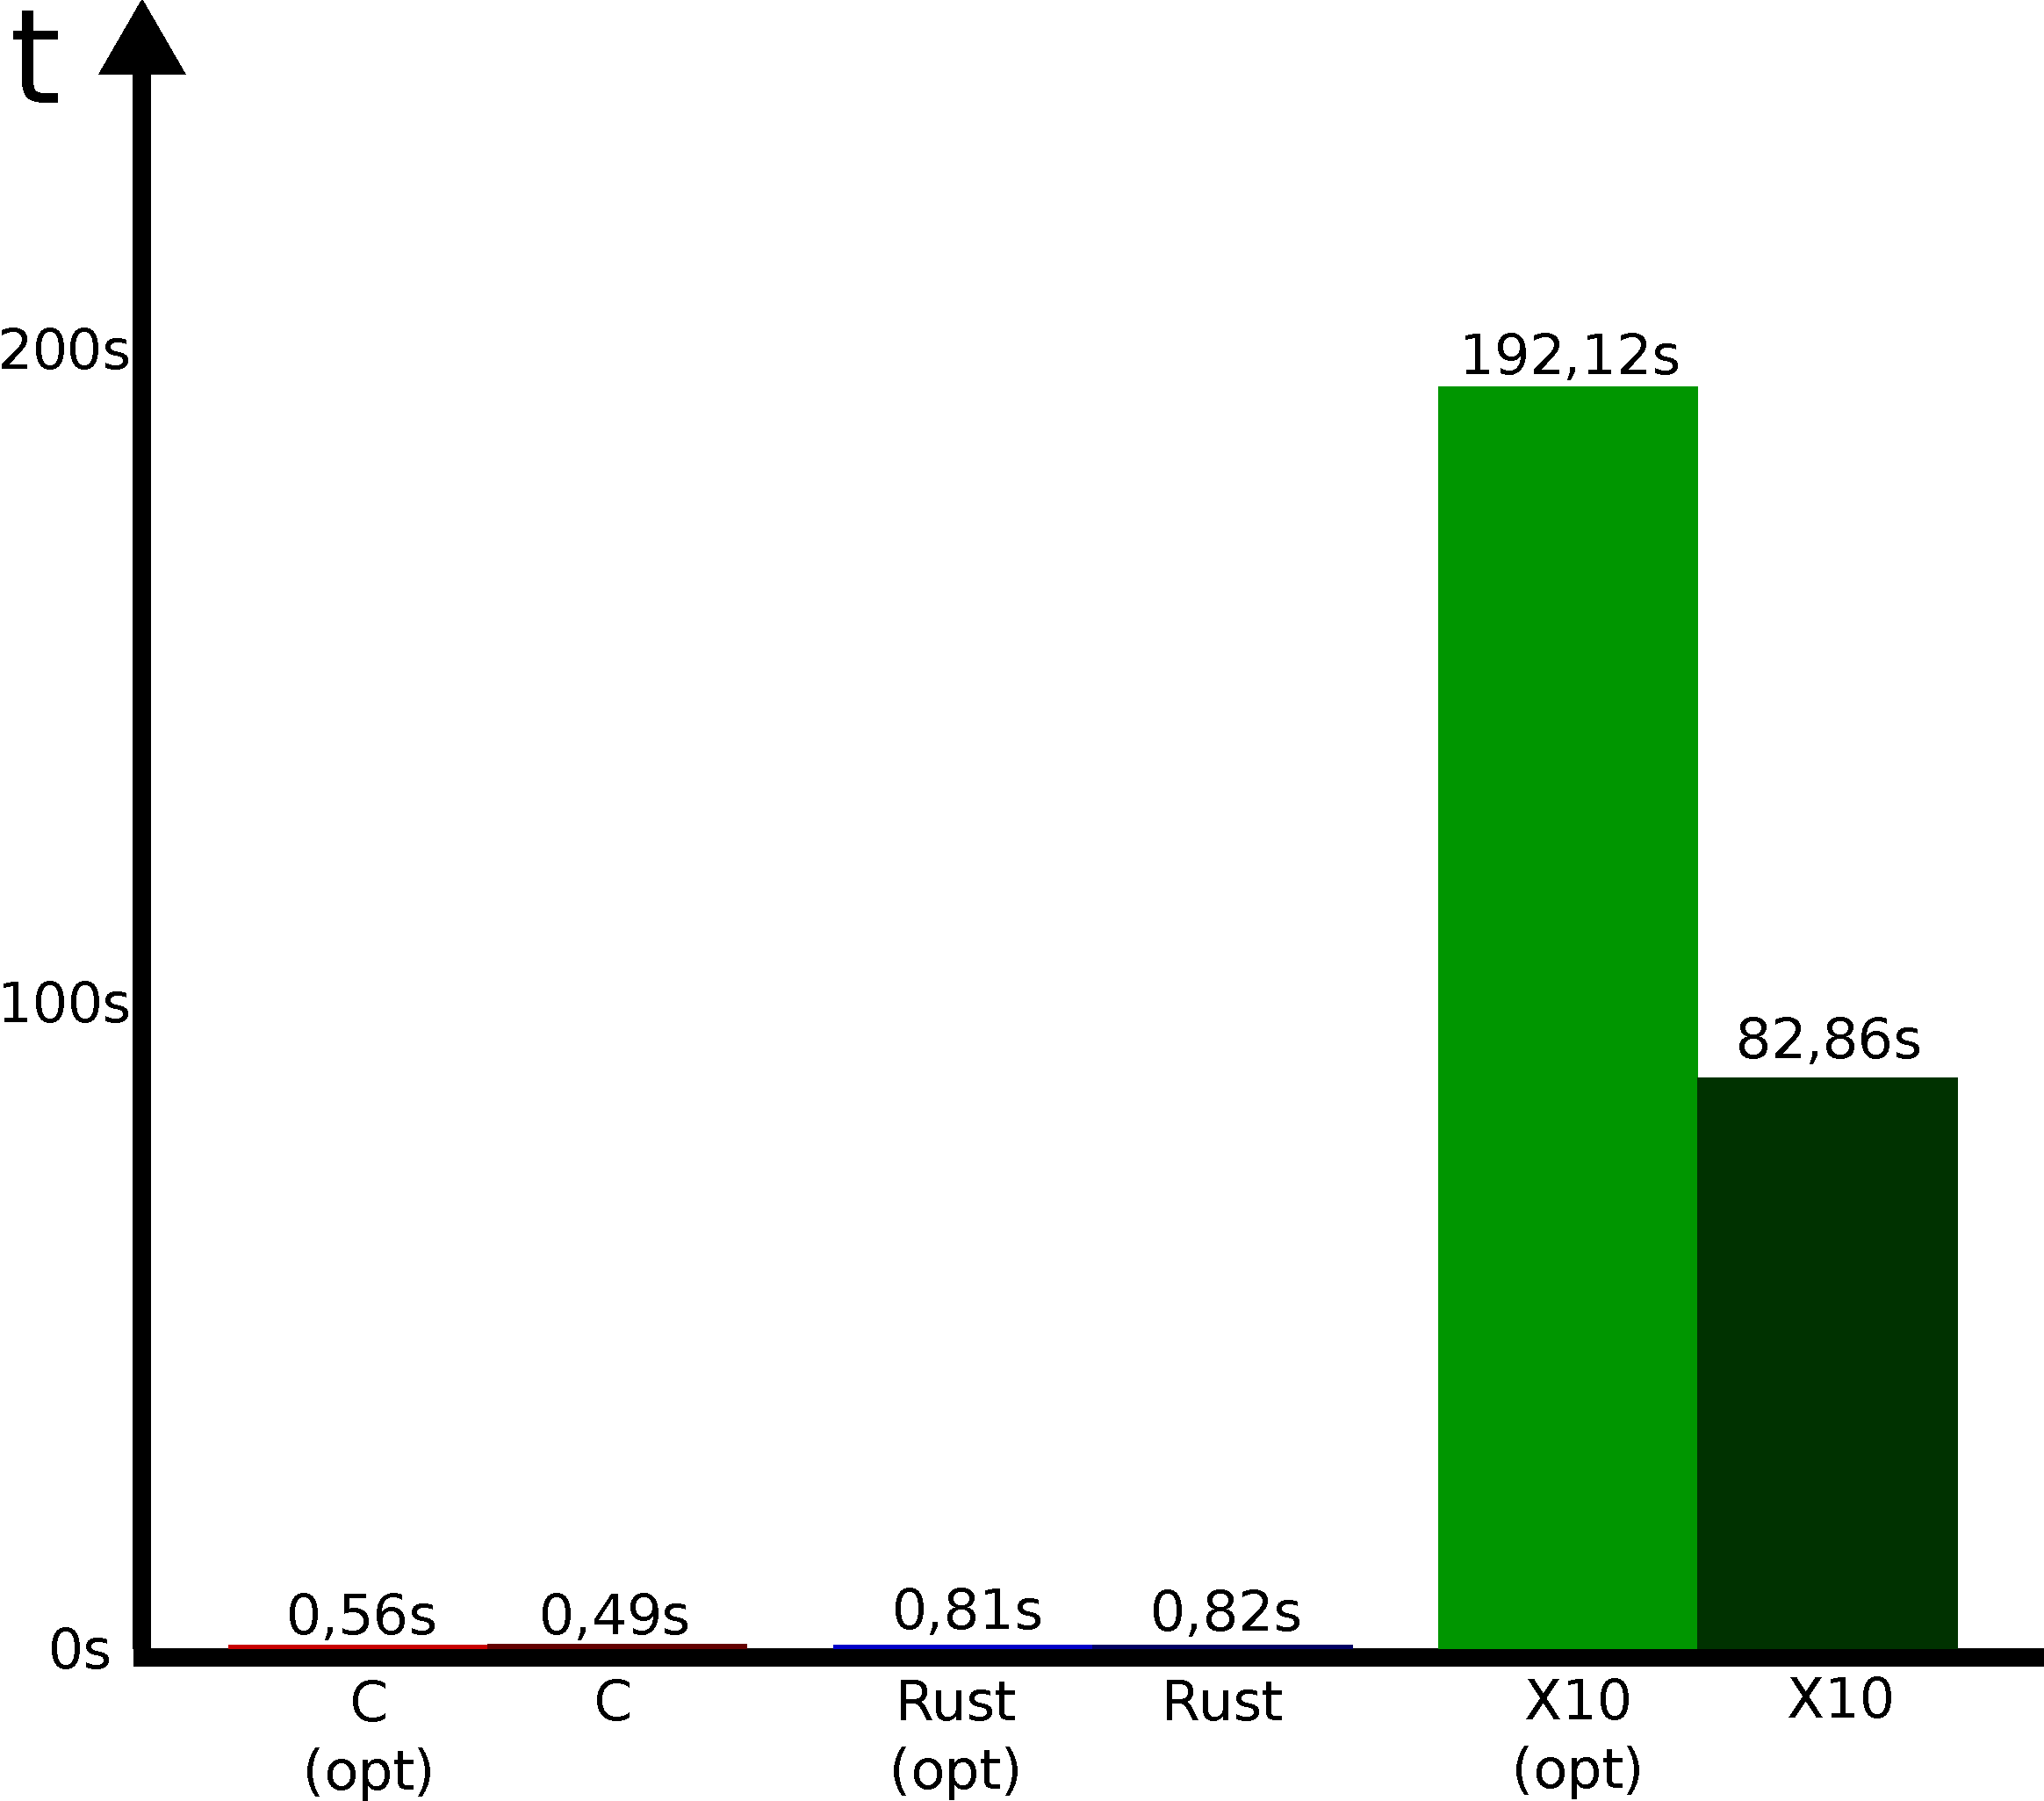
\includegraphics[width=0.55\textwidth]{images/compile-eval.pdf}
  \end{center}
  \begin{itemize}
    \item Zeitersparnis beim Kompilieren von Rust-Programmen im Vergleich mit X10-Programmen
  \end{itemize}
\end{frame}

\begin{frame}{Anlaufzeit}
  \begin{center}
    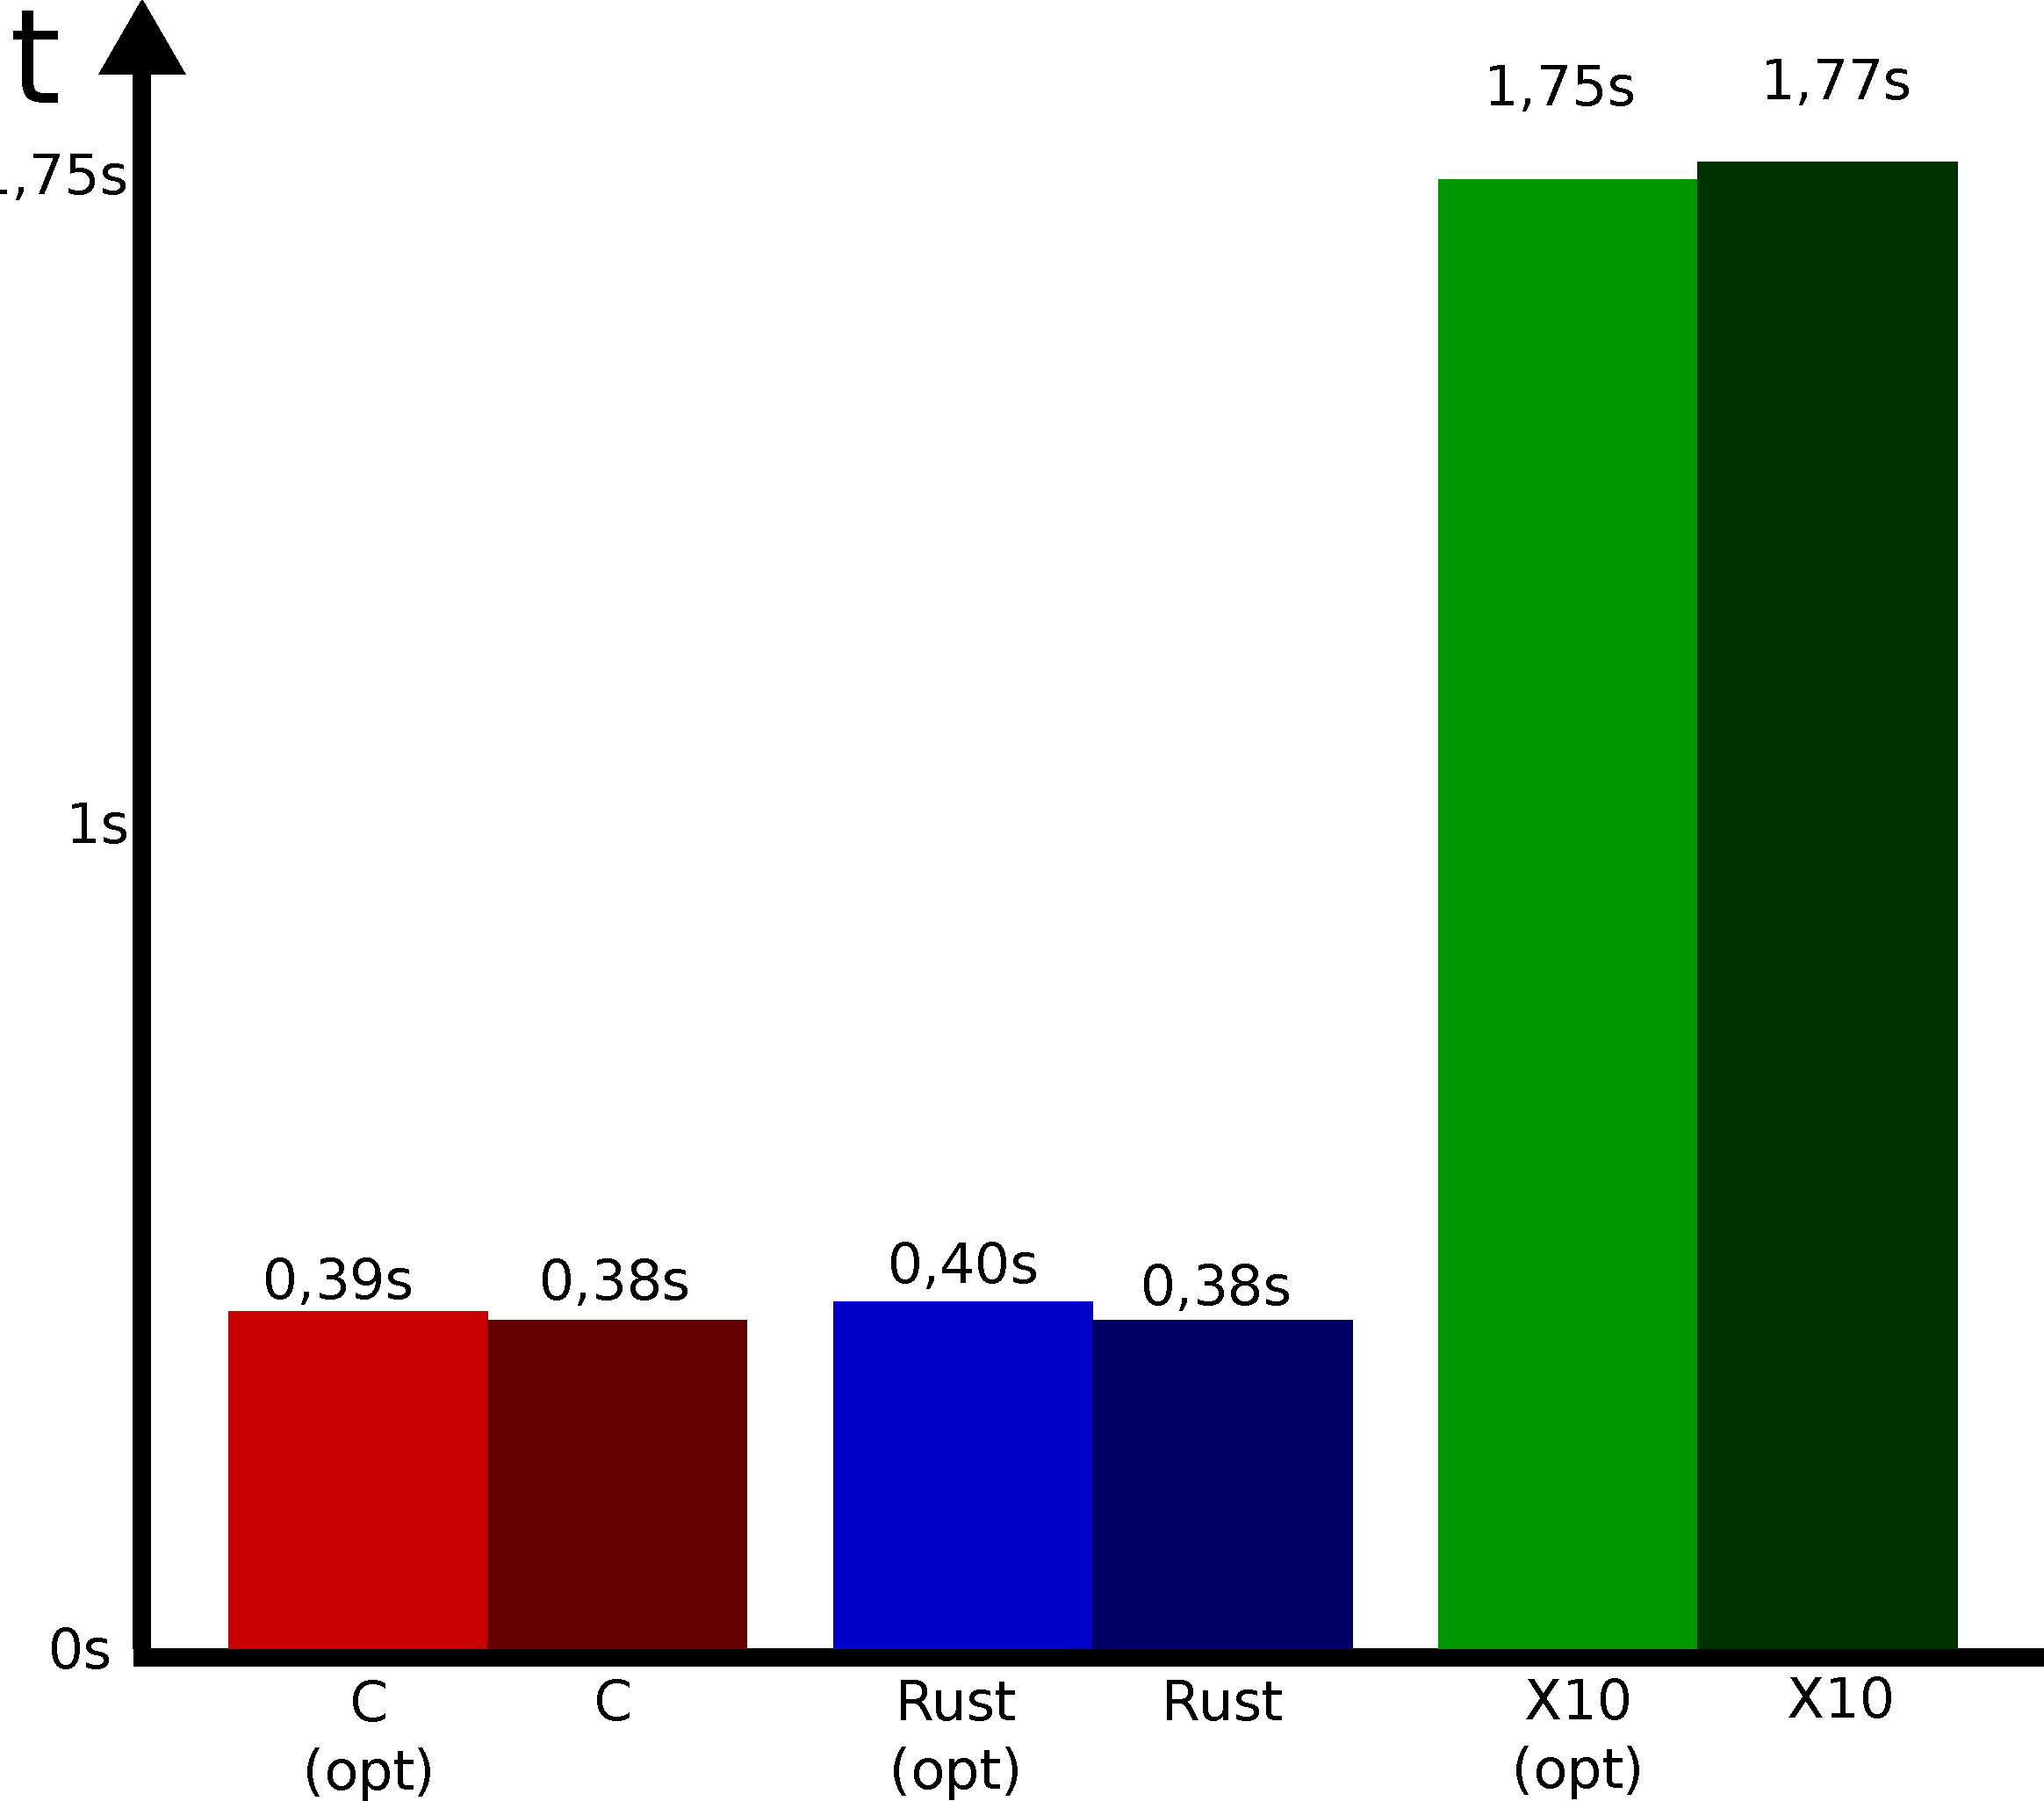
\includegraphics[width=0.55\textwidth]{images/startup-eval.pdf}
  \end{center}
  \begin{itemize}
    \item Rust und C benötigen ca. 1.4 Sekunden weniger um zu starten
  \end{itemize}
\end{frame}

\begin{frame}{Parallele Primzahlenberechnung}
  \begin{center}
    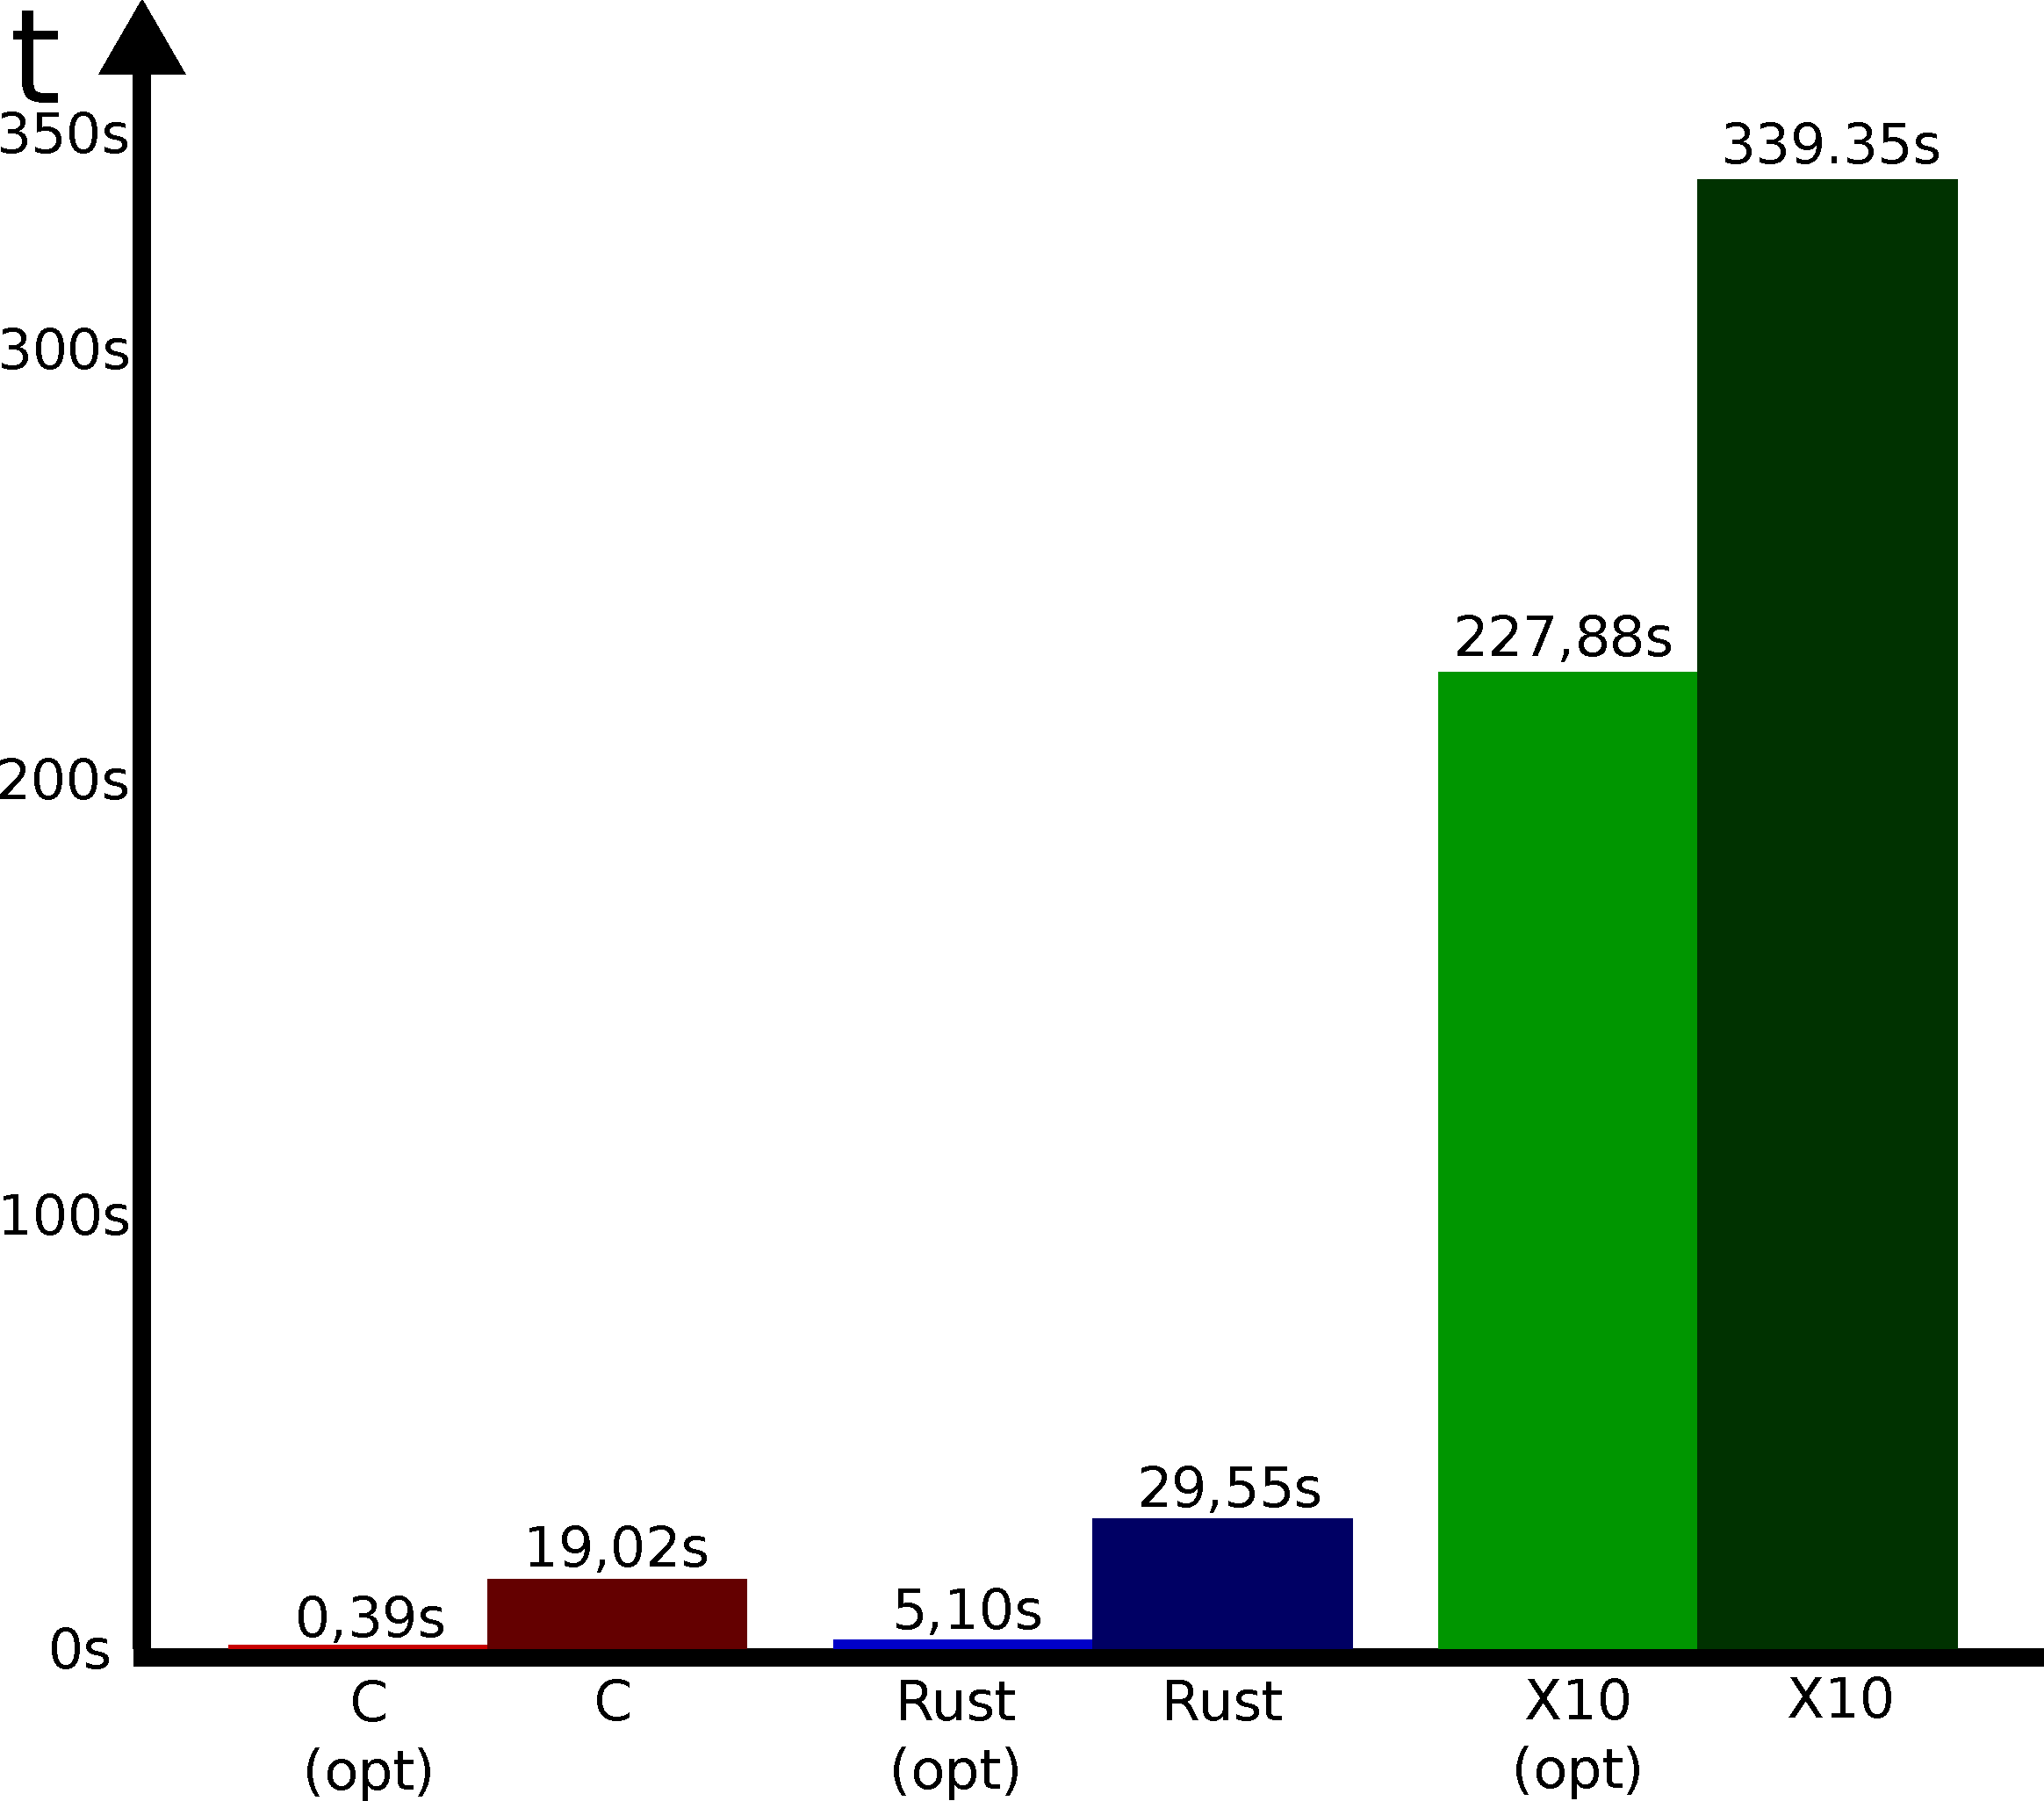
\includegraphics[width=0.55\textwidth]{images/primes-eval.pdf}
  \end{center}
  \begin{itemize}
    \item Rust weist bei Berechnung von Primzahlen keine Leistungsvorteile auf
  \end{itemize}
\end{frame}

\begin{frame}{Allokation von Objekten}
  \begin{center}
    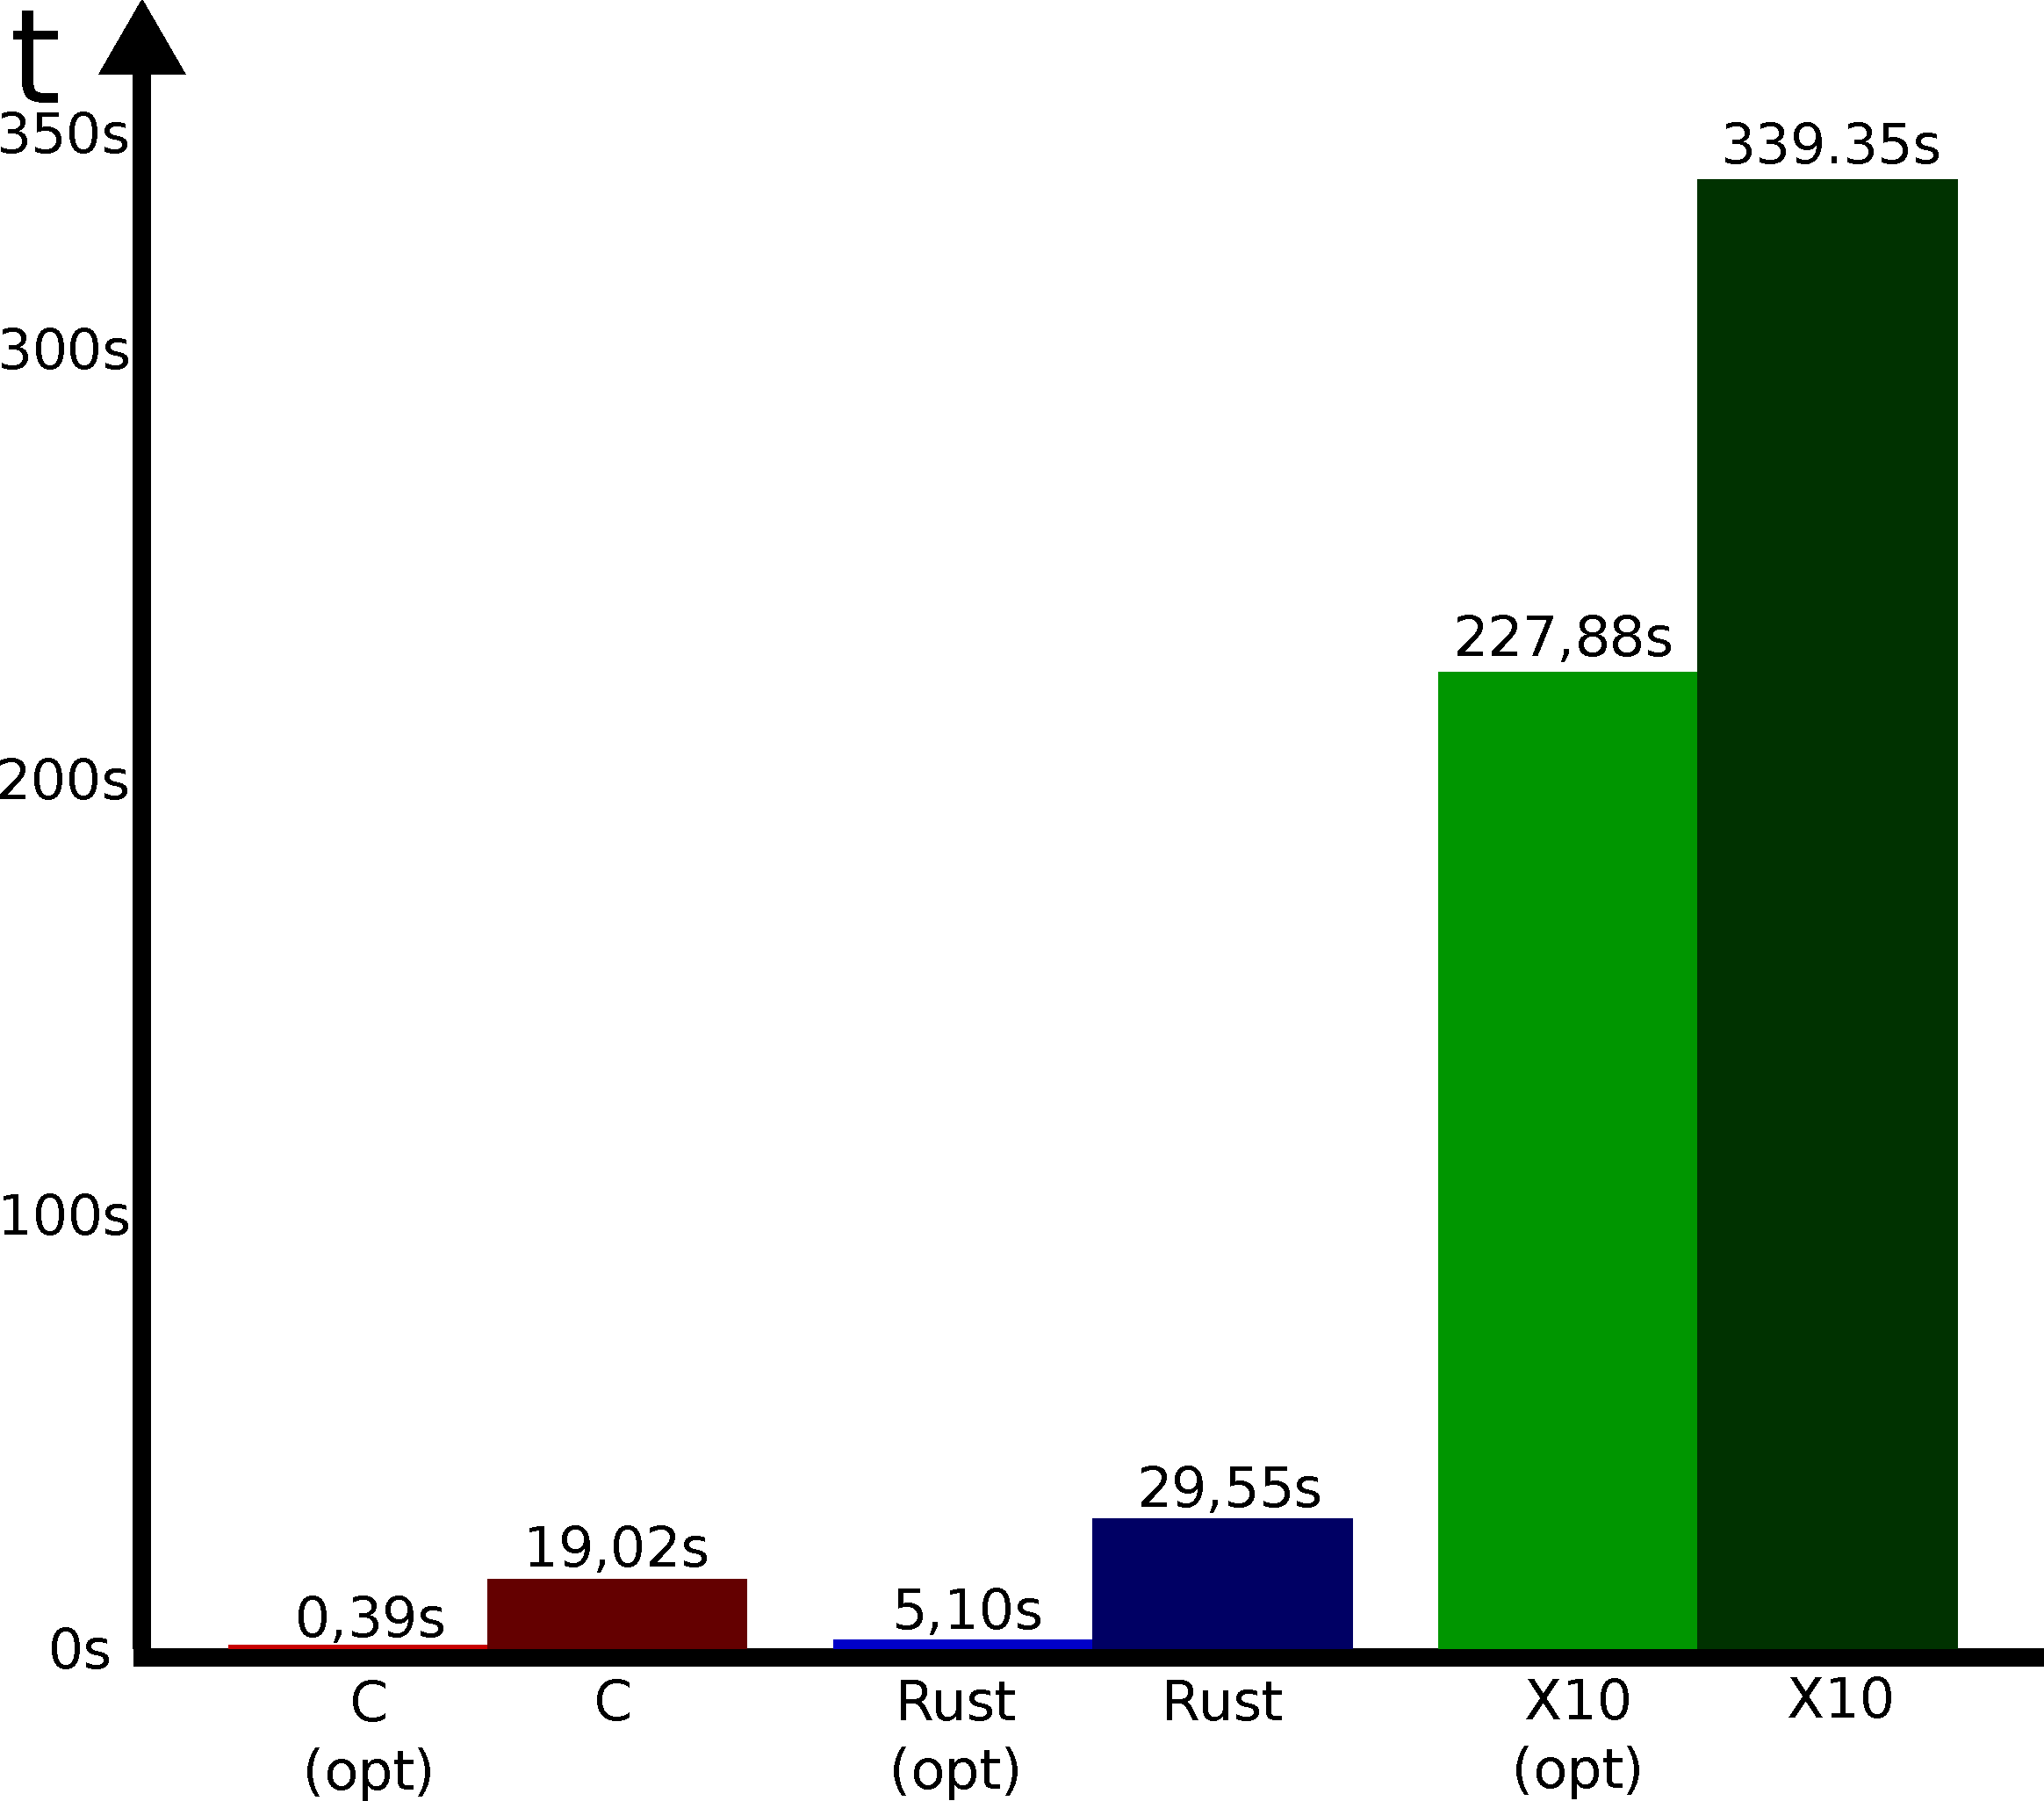
\includegraphics[width=0.55\textwidth]{images/garbage-eval.pdf}
  \end{center}
  \begin{itemize}
    \item C und Rust weisen eine mindestens 10-fach bessere Laufzeit als X10 auf
  \end{itemize}
\end{frame}